\documentclass[conference,compsoc,a4paper]{IEEEtran}
\usepackage{geometry}
 \geometry{
 a4paper,
 total={170mm,257mm},
 left=20mm,
 top=20mm,
 }

\usepackage[backend=bibtex]{biblatex}
\usepackage{array}
\usepackage[utf8]{inputenc}   % <<<<< Linux
\usepackage[nomain,acronym,xindy,toc]{glossaries} 
\usepackage{graphicx}
\usepackage{tabularx} 
\usepackage{float}

\usepackage{color, colortbl}
\definecolor{Gray}{gray}{0.9}
%Includes "References" in the table of contents
%\usepackage[nottoc]{tocbibind}

\bibliography{references} % or

\hyphenation{op-tical net-works semi-conduc-tor}
\loadglsentries[main]{xacronyms}

\newcolumntype{Y}{>{\centering\arraybackslash}X}
\newcolumntype{M}[1]{>{\centering\arraybackslash}m{\linewidth/#1}}

\begin{document}


\title{Hyper-linked Communications: WebRTC enabled asynchronous collaboration}

\author{\IEEEauthorblockN{Henrique Rocha}
\IEEEauthorblockA{Instituto Superior T\'{e}cnico\\}
\IEEEauthorblockN{Av. Prof. Dr. Anibal Cavaco Silva\\
2744-016 Porto Salvo, Portugal\\
henrique.rocha@tecnico.ulisboa.pt}
\and
\IEEEauthorblockN{Ricardo Pereira}
\IEEEauthorblockA{Instituto Superior T\'{e}cnico\\}
\IEEEauthorblockN{Av. Prof. Dr. Anibal Cavaco Silva\\
2744-016 Porto Salvo, Portugal\\
ricardo.pereira@inesc-id.pt}}

\maketitle

\begin{abstract}
The Hyper-linked communications concept applies much of the hypermedia concepts, widely used on Web content. This paradigm allows to synchronize, structure and navigate communication content integrated into voice and video calls.

Voice and image together can express emotions like no other medium can. With hypermedia concepts, we can add more value to conference calls.

\emph{WebRTC} technology allows real-time communications between web browsers without the need to install additional software. The nature of web browser applications already follows the hypermedia concept, which makes \emph{WebRTC} the ideal technology to apply the hyper-linked communications concepts.
The web browser platform provides an abstraction layer that makes it possible to create applications that run independently from the operating system.
The native support for \emph{WebRTC} in operating systems extends its usage to outside the web browser, allowing for the exploration of functionalities for which web browsers provide poor support, such as video recording and massive information storage.

Our goal was the development of an application targeted to the web platform, resorting to \emph{WebRTC}, that leveraged the hyper-linked communications by providing a conference environment enriched with multiple media types, collaborative text editors, time annotations, instant messaging and a mechanism to superimpose hyper-content to video.
\end{abstract}

\IEEEpeerreviewmaketitle

\section{Introduction}
\label{chapter:introduction}

\subsection{Background}
\label{section:background}

	As communications technologies appeared, we adapted the way we communicate. The purpose of this project is not the replacement of the current video and audio communications, but to enrich them with hyper-media content and make them a more natural and easy to learn process. 

	With the advent of WebRTC and its successive integration with web browsers, it became possible to develop video conference web applications without plugins, this presents a range of possibilities on what can be implemented using already existing web technologies.
		
    Furthermore, real-time communication applications can make a significant difference on business, education and health sectors by providing tools for developing teaching and learning online, teamworking and socializing web applications.

\subsection{Proposed Solution}
\label{section:proposed}

	Our goal in this project is to develop an application targeted to the web platform, resorting to \gls{WebRTC}, that leverages the hyper-linked communications by providing a video conference environment enriched with interactive and non-interactive discrete media types such as images, subtitles, forms and all types of content that can be added using \gls{HTML}5, \gls{CSS}3 and \emph{JavaScript} including continuous media types such as video, music and animations.

	One of the key features of this project is the ability to navigate in time in order to reproduce the conversation again or introduce hyper-content to it such as time annotations, interactive lists of topics and subtitles. In this context we also provide a simpler method for creating and synchronizing hyper-content using \gls{QR} codes.

	In addition to this conference environment, which provides different functionalities than traditional conference environments such as \emph{Skype} and \emph{Google Hangouts}, we also enable a collaborative text editor and a chat that supports sending time hyper-links and files to conference participants.

	Furthermore, another relevant feature is the possibility to compose multiple video streams into a single one, which enables adding more users to conference rooms without impacting on clients performance. Users can change to individual streams on demand or automatically to the talking users.
        

\subsection{Thesis Contribution}
\label{section:contribution}

Making it clear, this project aims to complement current audio, text and video communications in order to create rich and collaborative interfaces with the ability to add more content on a future time (\emph{e.g.} creating time annotations for improving content search) in order to increase its value. It is also important to highlight another goal of this project which is the ability to navigate in time by rewinding communications, fast-forward and jump to certain points.

	We have presented an architecture that can meet our goals, implemented the respective prototype and tested it with real users and performance benchmarks.

	According to Martin Geddes, the quality of the interaction worsens as the number of users increase\cite{geddes}. In our testing phases we will quantify and qualify the impact of increasing users on the interface and performance of our prototype. 

	All the problems faced during the development and limitations were reported on the thesis so that a future project better then ours can be easily and better developed.

\subsection{Outline}

This rest of this document is structured as follows:

\begin{itemize}

\item \textbf{Chapter \ref{chapter:relatedwork}} describes the previous work in the field.
\item \textbf{Chapter \ref{chapter:architecture}} describes the system requirements and the architecture for an Web Application that fulfills the goals of this thesis.
\item \textbf{Chapter \ref{chapter:implementation}} describes the implementation of our Web Application and the technologies chosen.
\item \textbf{Chapter \ref{chapter:evaluation}} presents the evaluation tests performed and the corresponding results.
\item \textbf{Chapter \ref{chapter:conclusion}} summarizes the work developed and proposes future work.
\end{itemize}

\section{Related Work}
\label{chapter:relatedwork}

One way to overcome the \gls{IPv4} address scarcity problem \cite{ipv4} was the development of a mechanism that groups multiple address into a single one, the machine that is assigned that address is then responsible for redirecting messages to members of its group using their private addresses, each connection in the private network is identified publicly by the same \gls{IP} address with a different port. This technique is known as \gls{NAT}\cite{rfc3489}.

\gls{NAT}s weaknesses are being exposing at the application layer, namely impacting applications that require direct communications between two private networks.

In order to implement an hyper-linked communication solution, several design decisions had to be made. The limitations imposed by the \emph{Internet's} structure, its protocols and a browser's capabilities are key factors to consider when implementing a solution that allows bi-directional communications, interactive media and collaboration environment.

Due to the use of \gls{NAT}, bi-directional communications between clients have different needs from request-response based communications between clients and servers.
This lead to the appearance of mechanisms such as \gls{STUN}, \gls{TURN} and \gls{ICE}, in order to bypass the limits imposed by \gls{NAT}.

\gls{STUN}, \gls{TURN} and \gls{ICE} \cite{natvoip} servers are a possible solution to overcome \gls{NAT}'s exposed weaknesses to applications that require communications between two private networks. 


When connection is established, \gls{WebRTC} came to simplify how audio and video are transmitted through web browsers. \gls{WebRTC} is an open source technology that defines a collection of standard protocols and \emph{JavaScript} \gls{API}s for web browser based real time communications without installing any additional application or plug-in. 

\gls{WebRTC} uses \gls{SDP} \cite{rfc4566} to define peer connection properties such as types of supported media, \emph{codecs}, protocols used and network information. An \gls{SDP} offer describes to other peers the expected type of communication and its details, such as used transport protocols, codecs, security and other.


Some operating systems such as \emph{Android}, \emph{iOS}, \emph{Linux}, \emph{OSX} and \emph{Windows} implement native \gls{WebRTC} libraries, extending the usage of \gls{WebRTC} to applications outside the web browser. This native support can help to implement applications that record video and audio streams for further playback.

However, \gls{WebRTC} by itself does not define how users get to know each other nor how information flows between users. For this reason, we have studied the multiple ways we could implement this \emph{get-to-know} mechanism which is known as signaling protocol.


  Signaling is the process by which applications exchange connection information about peers and servers, their capabilities and meta-data.
  In particular, \gls{WebRTC} does not implement signaling, as different applications may require different protocols and there is no single answer that fits all problems.
  As a consequence, multiple options are available for filling the missing \gls{WebRTC}'s signaling component, which can be performed using \gls{SIP}\cite{rfc3261}, \gls{XMPP}, \emph{WebSockets}, \emph{Socket.io}\footnote{\url{http://socket.io/}(accessed June 1, 2015).}, \gls{SigOfly}\cite{sigofly} or by implementing a custom protocol.

  One of \gls{WebRTC} signaling's requisites is bi-directional communication. The \emph{WebSocket} protocol allows bi-directional communications over a full-duplex socket channel \cite{rfc6455}, by other words it supports sending and receiving data simultaneously.

With the communications establishment issue solved, we had to discuss the different types of media and what can be done with each kind in order to increase the value of communications among users. In this context, we have studied solutions and libraries that allow us to implement our prototype with time manipulation features, collaborative text edition, record and playback interactive video. 

	\emph{Hypermedia} concept brings the possibility to organize and overlay multimedia elements into a nonlinear linear structure holding the promise of future technology and features. Languages such as \gls{SMIL}~\cite{hyval}, \emph{HyVAL}~\cite{hyval} and \gls{HTML} can be used to implement the \emph{Hypermedia} concept. Two examples of applications that captured our attention were \emph{HyperCafe}~\cite{hypercafe} and \emph{Hyper-Hitchcock}~\cite{hitchcock} which explored interactive video features.

  Using technologies that relies only on web standards, like \gls{CSS}, \gls{HTML}5, \emph{JavaScript} and \gls{SVG}, will make possible to develop an application that applies the hypermedia concept with the advantage of being compatible with a greater amount of web browsers.
  
\subsection{Extending collaboration tools with time manipulation}
\label{collab}

Real time collaboration applications have become a huge help on team tasks, providing a great boost on business, research and investigation velocity.

 Our first concern on real time collaboration applications is the data storage and representation. Storing multimedia content on a web client is not a viable solution because the local storage is limited to at most five megabytes per origin. Additional servers will be required to process and record the large amount of data generated by audio and video streaming.
 
\gls{KMS} supports streaming over \emph{WebRTC}. Another important component of \gls{KMS} is \emph{Kurento Repository}, which supports recording and playing directly from \emph{MongoDB}. That is important for providing a scalable media storage. 
	
     \gls{OT} technology was originally developed for consistency maintenance and concurrency control over distributed objects.
     \gls{OT} algorithms are mainly used in collaborative applications such as distributed document edition.

	Among mutiple \gls{OT} platforms and libraries we present \emph{ShareJS}\footnote{\url{http://sharejs.org/}(accessed June 2, 2015).}, \emph{TogetherJS}\footnote{\url{http://togetherjs.com/}(accessed June 2, 2015).}, \emph{Goodow}\footnote{\url{http://realtimeplayground.goodow.com/}(accessed June 2, 2015).}, \emph{Etherpad Lite}\footnote{\url{https://github.com/ether/etherpad-lite}(Accessed 20 March 2016)} and \emph{otJS}\footnote{\url{http://operational-transformation.github.io}(accessed March 10, 2016)}.


	\emph{otJS} is a \emph{JavaScript} library that only implements operation transformations over plain text on the client side and requires implementing the content's persistent storage. Besides this drawback, this library is very flexible because it is not tied to a specific database or server side technology.
        


\section{Architecture}
\label{chapter:architecture}

Taking into account the goals of this project and all the technology presented so far. Our proposal is the development of a web application that provides communication and collaboration features in real-time.

\subsection{Requirements}
In a general way our system's goal is to provide a multi-party video and audio conference environment that supports chat, time manipulation, collaborative text edition and hyper-content creation.

%RP isto pode ser muito expandido. Podes começar por descrever os goals (mais alto nível): audio e video conferência multi-party, possibilidade de rever o que foi dito antes, chat, etc etc.
% Só depois traduzes isso em requisitos, tanto funcionais como não funcionais
% Depois apresentas a arquitectura, fazendo um paralelo entre os módulo e escolhas realizadas e quais os requisitos que cada um deles satisfaz. 

For our system, our application must provide: a simple way to send instant text messages to the conference participants, ability to recording and playback recorded video including all the hyper-content displayed at that time, mixing multiple user streams into a single stream, create annotations associated to a specified time, allow users to superimpose hyper-content to video given a range of time, search every objects related to a conference room such as hyper-content, time annotations and users, share files and time links among users, sound detection for showing the current speaker, provide a collaborative text edition tool, interpret \gls{QR} codes in order to ease content creation and support database replication.
%RP capacidade de lidar com NAT

	Moreover we allow clients to discover chat rooms and other clients by navigating on the web pages provided by our web server. In addition users can create rooms for multi-party audio and video communication communication which is achieved by using \gls{WebRTC}'s \emph{PeerConnection}.
        %RP falas em peerconnection, mas na figura 3.1 apenas há um cliente, o que obviamente impede mostrar a comunicação entre peers.
        %RP acho que podes fazer outro diagrama com a comunicação entre os vários componentes, onde apareceriam vários clientes. A aí indicas o tipo de ligação entre cada par de componentes (HTTP, PeerConnectino, websocket, MediaStream ...)
        
\subsection{Modules}
In this section we present the several modules that were designed in order com fulfill the set requirements.
	Figure~\ref{fig:modules} presents the structure of our system which was divided into six modules:


\begin{figure}
	\centering
	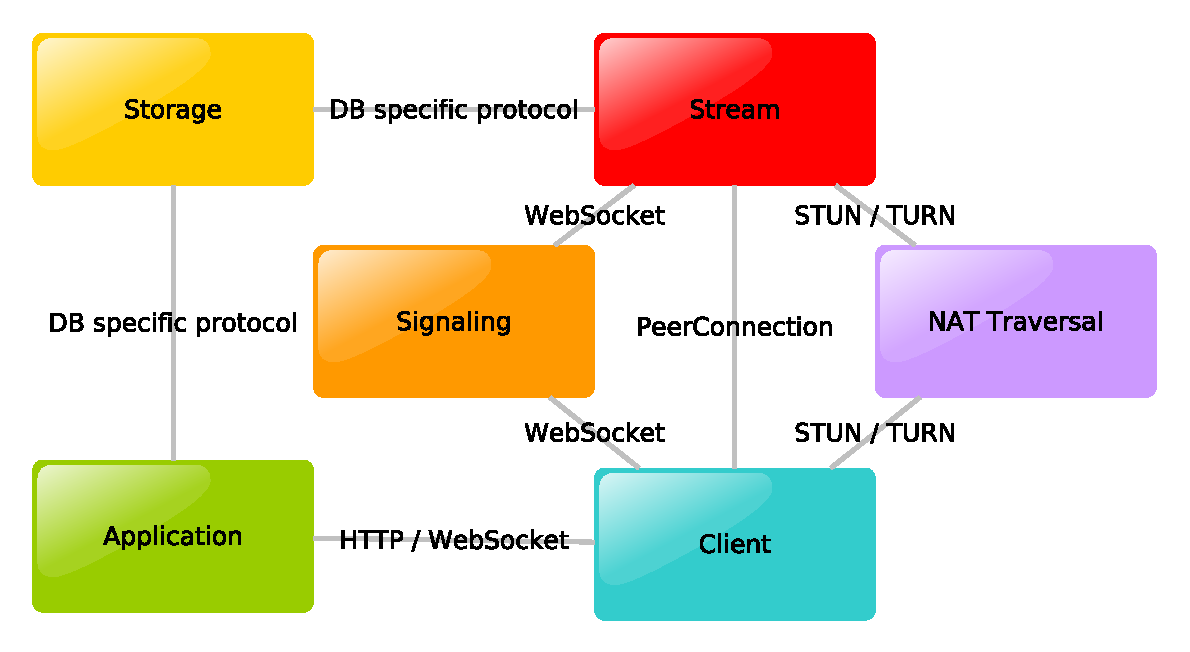
\includegraphics[width=\linewidth]{figures/modules.pdf}
	\caption{System Modules}
    \label{fig:modules}
\end{figure}



\begin{itemize}

\item \textbf{Application module} - responsible for providing information about the relevant modules (\emph{NAT Traversal} and \emph{Signaling}) and user interface to the \emph{Client} in the form of web pages in \gls{HTML} and \emph{JavaScript} libraries through \gls{HTTP}.
 
\item \textbf{Signaling module} - responsible for \emph{Client} and \emph{Stream} coordination which will be performed using \emph{WebSockets}.

 \item \textbf{NAT Traversal module} - \gls{STUN} and \gls{TURN} techniques used by \emph{Client} and \emph{Stream} modules during the \emph{Signaling} phase which ends by establishing the connection between them.

 \item \textbf{Stream module} - responsible to deliver and receive multimedia content from the \emph{Client} using \gls{WebRTC}. 

 \item \textbf{Storage module} - provides two main functionalities: store the model information and media recorded. This is the single module responsible for persistent storage. It stores user and communication data as well as all the data required among user sessions. It is also use to store all the communication streams, so that they can be viewed later.

 \item \textbf{Client module} - responsible for the interaction with the user.

\end{itemize}

%RP Acho que podes escrever muito mais sobre cada componente. Isto está muito curto. Fala de algumas das funções que proporcionam. Vê o que fiz com o Storage Module

%RP também podes fazer um diagrama com vários utilizadores e mostrar quais os streams que vão de e para cada um (mostrar a mistura de som, video, etc).

 
\subsection{Implementation Proposal}
The infrastructure is composed by: web server, stream server, signaling server, database and video repository.
%RP tens da fazer o paralelo entre isto e os componentes apresentados na secção anterior. O mesmo com a imagem, que parece não estar relacionada. Podes colocar os elementos na mesma posição, ou dentro das caixas da imagem 3.1

\begin{figure}[H]
	\centering
	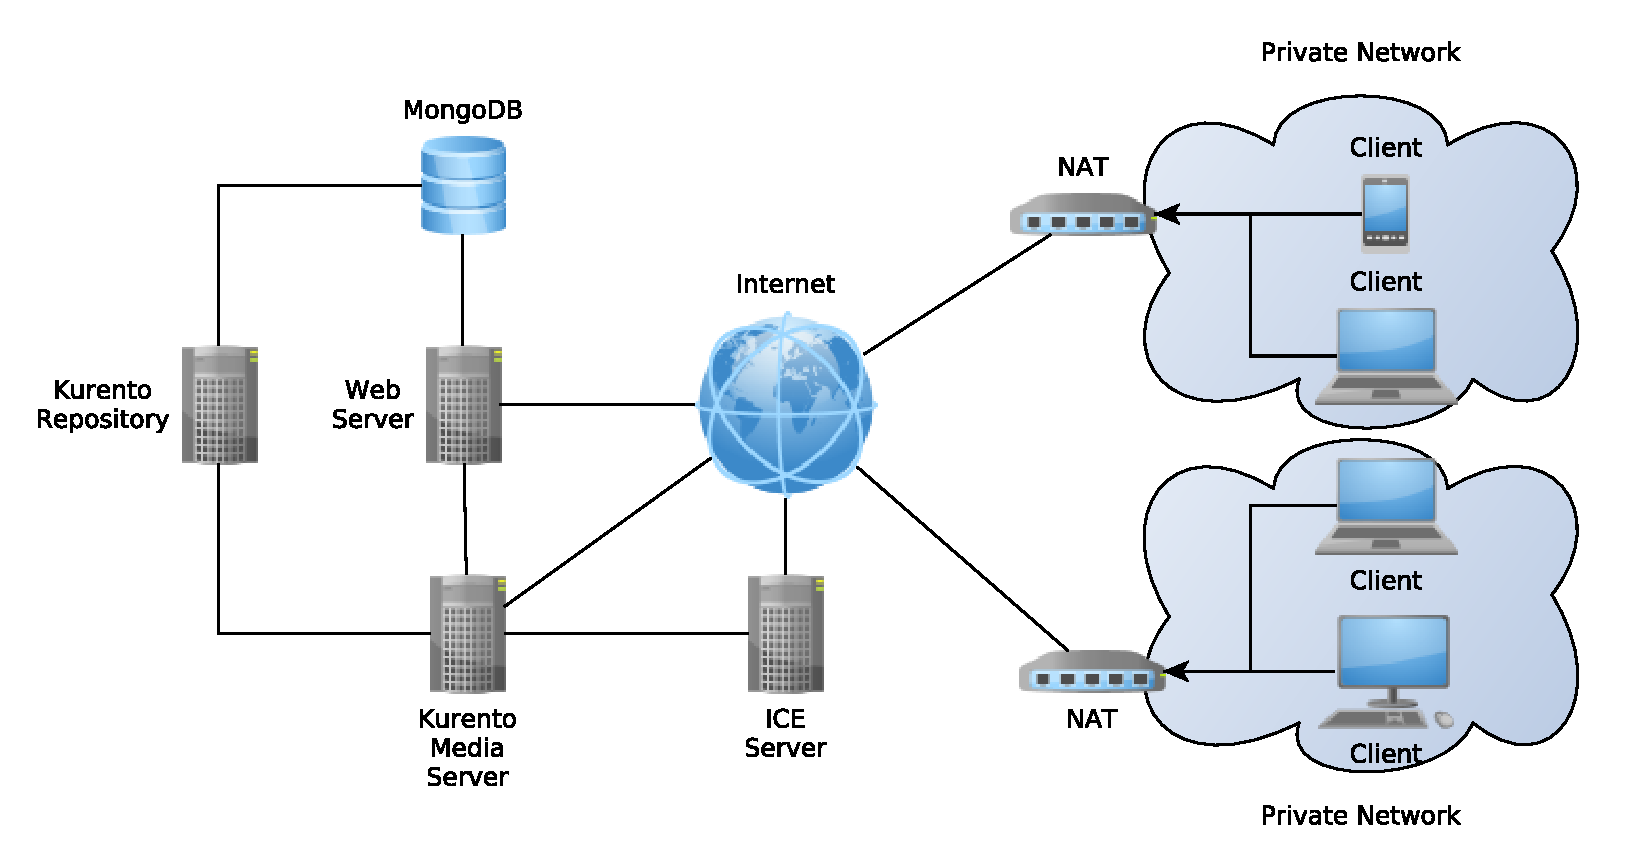
\includegraphics[width=\linewidth]{figures/infrastructure.pdf}
	\caption{System Infrastructure}
\end{figure}

In order to simplify our solution, we propose that the \emph{Application}, \emph{Signaling}, \emph{Stream} and \emph{Storage} modules be implemented within the same server application, so it could be easy to deploy as a single image. To this set of modules, we often call \emph{backend}.

	\subsubsection{Security and authorization}

Having established that the \emph{backend} modules are placed in the same machine, that helps controlling which resources the client has permission to access as those modules are seen as a private network.
%RP na mesma ``server application'' ou ``machine''? São coisa diferentes! Apresentas vantages de instalar tudo na mesma máquina mas não falas das desvantagens. Menor escalabilidade parece-me ser logo uma delas. Na figura 3.2 aparecem várias máquinas!

To qualify the above we provide public access to \gls{HTTP} server ports, maintaining the access to other components restricted through firewall rules.
%RP qualify?
%RP Imagem com firewall e estes portos? Mas isto já me parece muito detalhe de implementação.
In relation to the database there is no directly access from the outside. All the database information is accessed via our application server which validates the permissions of users on our system.

On the other hand, the access to our streaming servers is also restricted, but clients can connect to them after concluding the signaling phase. This signaling phase may or not proceed in function of the client access permissions. For example, if a user is trying to access a private conference room that he is not a member of nor has an invitation link for, the signaling server refuses to start the signaling phase and the user cannot access the streaming server.

The placement of our streaming servers inside a \gls{NAT} also has an important role with respect to external misuse prevention. Otherwise, placing our streaming servers could allow external clients to perform their own signaling protocol and, as a consequence, use our infrastructure without our consent.

\subsubsection{Client connections}
	Although the delegation of processing work to clients can improve our system's scalability, we are concerned about using the least resources possible on the client side, as huge resource consumption may drain battery very fast or may even be impossible to run on mobile devices. We are aware that streaming video from clients is already a very intensive task which we cannot avoid but can improve by delegating the most intensive tasks to our servers. 


	In this context, with a centralized approach, each client must only have one \emph{PeerConnection} to our streaming server and content shown to them is changed on demand either being it an individual or a composite view. Otherwise clients could follow a peer-to-peer connection which would result on maintaining more connections and performing the composition of videos on client side.

	The composition of streams on client side is performed by receiving streams with the best quality possible but, due to undersizing the video of clients into a smaller region, this would result on wasting bandwidth on a quality that is not needed.

	Although the peer-to-peer approach could be used on our system, we conclude that we need to record the video on our streaming server because web clients have a very limited storage and peer disconnections may result on recorded video loss. 

	The same can be concluded to instant message delivery, each client must have only one \emph{WebSocket} connection to the application server which consequently relays the messages to other users.

	Relaying instant messages from clients through the our web servers is easier if all clients are connected to the same server because all messages can be directly delivered without sending messages across multiple web servers. 

	In the context of this thesis, we will not implement sending messages across web servers but, in order to allow our system to scale, we will consider that all conference participants are connected to the same server and our system is scaled by having conference rooms distributed across different servers.

\subsubsection{Software choices}

Furthermore, we have taken into account the compatibility between the streaming server, database and the operation transformation solutions, in order choose the appropriate framework to implement our web server.
%RP esta secção devia começar aqui, a explicar a escolha das tecnologias/produtos a usar em cada componente. O que tens antes são pormenores que só faz sentido discutir no final. Tens de ir sempre do mais geral para o mais detalhado.

We have decided that our solution must use \gls{KMS}. Our web server could be implemented easily with \emph{NodeJS} or \emph{Java} due to the fact \gls{KMS} provides clients for both technologies. But others could also be used as \gls{KMS} also exposes their \gls{API} via \emph{WebSockets}.

Due to the fact we are going to use \gls{KMS} as streaming server solution, we could choose \emph{NodeJS} or any \emph{Java} based web framework for implementing our web application server. We have decided to implement our web server with the \emph{PlayFramework}\footnote{\url{https://www.playframework.com/}(acessed March 25, 2016)} using \emph{Java} because of our previous experience with it.

By default, \emph{Kurento Repository} is implemented over \emph{MongoDB}, for convenience our storage model will also use the same database.

Importantly, for the collaborative text editor, we have chosen \emph{OT.js} due to its server and storage implementation choice independence.

For the \emph{NAT Traversal} module a public \gls{STUN} server can be used for testing our solution. Nevertheless, we recognize that for a production environment we would need to maintain our own \gls{TURN} servers in order to ensure connectivity to all clients.

Not less important, on the client computers, both \emph{Mozilla Firefox} and \emph{Google Chrome} could be installed as web browsers. As such, both should be supported. Libraries such as \emph{jQuery}, \emph{Bootstrap}, \emph{Adapter.js}, \emph{OT.js} can be downloaded from the web server and executed on the client side using any of these two browsers.
%RP relembrar que o IE e o Safari não suportam webrtc?

\begin{table}[H]
\centering
	\caption{Application Architecture}
	\label{table:apparch}

\resizebox{\columnwidth}{!}{%
    \begin{tabular}{cccccccc@{}m{0pt}@{}}
	\hline 
	\multicolumn{8}{|c|}{\cellcolor{Gray}Application}  &\\[12pt]\cline{1-5}\cline{7-7}
	\multicolumn{1}{|c|}{jQuery} & \multicolumn{1}{c|}{HTML5} & \multicolumn{1}{c|}{CSS3 (Bootstrap)} & \multicolumn{1}{c|}{Signaling} & \multicolumn{1}{c|}{ot.js} & \multicolumn{1}{c|}{\cellcolor{Gray}} & \multicolumn{1}{c|}{adapter.js} & \multicolumn{1}{c|}{\cellcolor{Gray}} &\\[12pt]\hline
	\multicolumn{1}{|c|}{HTTP} & \multicolumn{2}{c|}{User Interface}  & \multicolumn{3}{c|}{WebSocket}    & \multicolumn{2}{c|}{WebRTC}      &\\[12pt]\hline
	\end{tabular}
}
\end{table}

%RP acho interessante o que queres fazer aqui mas acho que está mal conseguido. A linha de baixo, devia ter coisas ao mesmo nível, o que não aconteçe.
% Qual a razão para HTTP estar por baixo do jquery e user interface estar ao lado?
% Sugiro colocar a applicação no meio e as várias interfaces (webrtc, websocket e http) uma de cada lado (esquerda, baixo e direita), indicando o que fica do outro lado (outro cliente, servidor web, servidor stream, etc)

Table~\ref{table:apparch} presents the application architecture and the underlying technologies seen from the user's perspective. \emph{Adapter.js} and \emph{jQuery} will ensure that our application is compatible with the most popular web browsers.
\emph{Bootstrap} will be used to make the user interface more appellative and responsive. With \emph{Bootstrap} it is quite easy to develop applications that adapt to mobile devices with different screen sizes.
%RP bootstrap não aparece na figura!

With respect to displaying content, the synchronization between multimedia elements will be performed through chains of \emph{JavasSript} events or by specifying the interval of time which time content must be visible. Other animations can be implemented with \gls{SVG} embedded on \gls{HTML}.
%RP Caiu do céu! Tens de explicar e ligar melhor a sequencia de texto

\section{Implementation}

\subsection{Data Model}

The data model is a critical component of our solution, as a badly designed model can imply serious difficulties when implementing new features that are not part of the plans. During the course of this project, we had to redesign the model more than once in order to support new features.

In order to offer all the functionalities that we promise, some information about objects must be persistent such as users, groups,relations among users, group memberships, messages, hyper-content, recordings and collaborative editor state. For designing our model we have taken into account generic programming techniques. We observed that operations like searching for an object were quite repeated across different types of objects. 

\subsection{Signaling Protocol}


Although we have mentioned that the signaling protocol is used to establish connections between peers, on our system our media server (\gls{KMS}) is a peer that receives video streams and sends to its connected clients. 

After the web application server validates the user access, the signaling protocol allows the users to directly connect to the \gls{KMS}, which is placed in a private network, and lets the application server and users negotiate media types and encoding information to use during the conversation.

Our signaling protocol consists of sending and receiving \gls{JSON} formated messages over \emph{WebSockets} by both the application server and the client. 


When a user enters a group conference, after the page is completely loaded, a WebSocket is created to maintain a connection with our web servers. 
But before creating the web socket, we must identify the user and check if he has permissions to participate in the conference. The user identification is done by retrieving the session id from the cookie provided by the user-agent (web browser) through the \gls{HTTP} headers.
%RP não é bem o user que fornece o cookie. é o user-agent (browser). Convém ser preciso.
%HR done
The Web application server retrieves all the information needed from the database in order to check if the user has permissions to join that conference room. It is important to save the user identification before the \emph{WebSocket} connection is created because, after the handshake is performed by the \emph{WebSocket} protocol\cite{rfc6455}, the \gls{HTTP} context is lost.
%RP socket -> websocket?

At this stage, the web application's user is asked if he wants to share its camera and microphone, share screen or just receive streams from the server. 

If the user decides to share his camera or screen the user agent creates an offer, sets a \emph{local session description} to its \emph{PeerConnection} and sends it through the WebSocket to the Application Server.

The server receives and processes the offer and sets the \emph{remote session description} to its client associated \gls{WebRTC} endpoint. Then a \emph{local session description} is created on the server and sent back to the client, after that the server tries to gather \gls{ICE} candidates.

The client receives the server answer, sets the \emph{remote session description} and gets the ice candidates from the \gls{ICE} server.
%RP tens ``ice'', ``\gls{ICE}''. Acho que também já vi ``ICE''. Convém ser sempre igual!

Subsequently, after a while both the server and client receive the \gls{ICE} candidates that allow the client to connect directly to \gls{KMS} and vice-versa. The candidates are received at the client which sets them to its \emph{PeerConnection}. The same is done on the server which receives the \gls{ICE} candidates from the client and propagates them to \gls{KMS}.


An \gls{ICE} candidate contains an \gls{IP}, port, used transport protocol and an attribute named \emph{sdpMLineIndex} that is used for mapping to the \emph{remote session description} media type.
When a connection is established, the user and server start to interchange stream data but other \gls{ICE} candidates may arrive with better connections.

Having the media session established, the server starts to record any received stream and the client creates an \gls{URL} correspondent to the stream location.

\subsection{Stream Recording}
 Initially we experimented with local recording and synchronizing with our servers. Even thought it got it to work, it consumed to much bandwidth. We then tried recording on server side.

	One of our concerns during the development of our solution was the storage scalability. Saving files directly into the file system would require an extra effort to distribute and replicate files among servers. For that purpose, the \emph{Kurento} team developed \emph{Kurento Repository}\footnote{\url{http://doc-kurento-repository.readthedocs.org} (accessed on 17 March 2016)} which is based on \emph{MongoDB}.


	With server side recording, the user would maintain always the same stream \gls{URL} even if it is playing real-time video or reproducing recorded video. It is \gls{KMS} that sends different content through that stream. When a user desires to play recorded video, a \emph{webSocket} message is sent specifying the time and the intended user id. The server performs the calculations in order to find a block that intersects the requested time, plays it and when finished, the next part is automatically played without the user intervention.

%RP não falas nada sobre chats, etc! Não há signalling para isso?
%HR não, só video e audio, chat é websockets


\subsection{Hyper-Content}

	Our system supports creating superimposed content to video, which is achieved by creating \gls{HTML} tags on top of the video  with the same size. The decision of which content must be displayed to each user is performed by our content scheduler which uses the user's current time in order to synchronize which content is shown or removed from the user interface.

	In order to create content, the user has the option to write simple movie captions without writing any code, otherwise, as mentioned before, it can write \gls{HTML}, \gls{CSS} and \emph{JavaScript}.

	As manually content insertion is a laborious task that can be realized after the video is recorder, we provide an alternative mechanism for real time introduction of superimposed content.	In order to help the content creator to introduce and synchronize its content in real-time, we allow the user to encode its content into \gls{QR} codes and show it to the camera in real time.


\subsection{Collaborative editor}

Our collaborative editor is a simple text editor that is synchronized with all participants within a conference room implemented using \emph{ot.js}.

The state of our collaborative editor is not saved on the database every time it changes. Instead, the users just synchronize the editor content among themselves using the application server to relay editor changes and save on demand.

\section{Evaluation}


\subsection{Tests Objectives}

  We have tested our solution with real users for a better understanding of their difficulties and what can be done in order to improve our solution's usability.

  We have also tested the performance of our solution by measuring the used resources. Those performance tests are crucial to ensure that our solution is in fact stable and users can use it endlessly without decreasing the quality of their experience. 


  \subsection {Performance Tests}

      In order to benchmark our system, we have implemented a small \emph{Python} script using \emph{psutil}\footnote{\url{https://github.com/giampaolo/psutil} (Accessed March 27, 2016)} that collects with a periodicity of one second: CPU, physical memory information relative to each running process and network usage relative to each interface. 

      The performance test scenario that we have defined consists on two phases, the first phase consists only on having users, with similar computer and network specifications, entering sequentially on the conference room. The second phase consists on the users leaving the conference room. Each event, joining and leaving, occurs with intervals of one minute in total of thirteen minutes (780 seconds).
  
      From the media server perspective if there are $n$ clients connected, each of them sending and receiving one stream, it is expected that server sends and receives also $n$ streams. As such, we expect that the amount of network traffic increases linearly as users join a conference room. Figure \ref{fig:test_full_features_net} confirms our expectations. Each vertical yellow line represents one event: the first seven events are users entering the conference room, the next ones represent users leaving the conversation. 
     

\begin{figure}
  \centering
  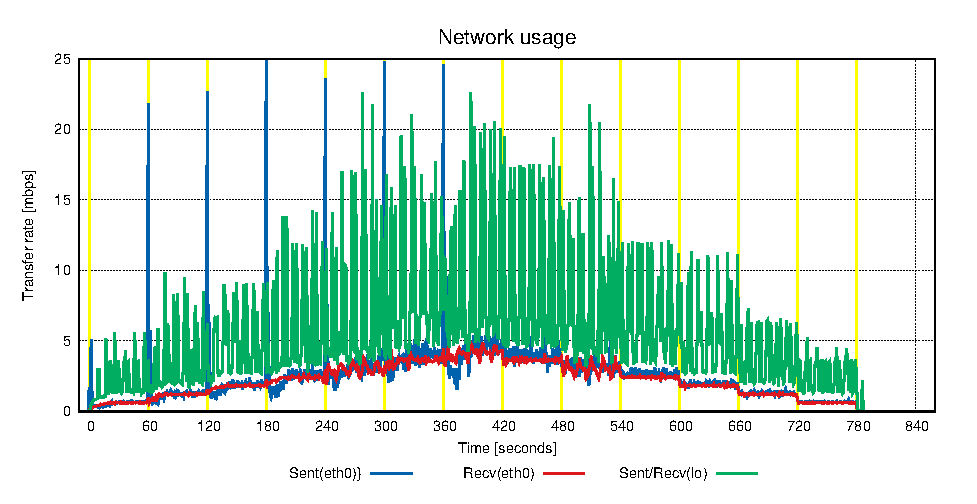
\includegraphics[width=\linewidth]{stats/test_full_features_net.eps}
  \caption{Network usage after implementing all features}
  \label{fig:test_full_features_net}
\end{figure}


      The blue peaks are caused by the signaling phase and web page downloads, including resources such as images, stylesheets and javascript files. 
      The green peaks are caused by video and audio being transfered between \gls{KMS} and \emph{MongoDB} through \emph{Kurento Repository}. Each peak occurs every time a block of video is recorded, which in this case is every ten seconds. 
      The recordings are synchronized so all user and mixed blocks start and end at the same time. That is why the amount of work done every ten seconds accumulates, and because this is performed locally, the maximum transfer rate is limited by the performance of the memory as buffers are written to buffers then to disks. 
      Sent data transfer rate has no significant peaks as \gls{HTTP} requests and signaling information contains little information.

	With this results we conclude that if we want to scale our storage solution using the \emph{MongoDB}'s cluster configuration, both \emph{Kurento Repository} and \gls{KMS} should be installed on the same machine because the loopback interface can handle bigger transfer rates than the remaining network interfaces. Installing the repository on the same machine as a database node does not ensure that recorded videos are stored in the same machine, for this reason we would prefer installing \gls{KMS} and \emph{Kurento Repository} on the same machine.





On the other hand, Figure \ref{fig:test_client_net} shows the respective network usage on the client side during our test case. We observe that in the first seconds the client adjusts the video quality it sends to \gls{KMS}. Whenever a new client enters the conference, we observe that \gls{KMS} decreases the video quality in order to instantaneously integrate a new user into the conference room. After a while, \gls{KMS} realizes that the network can handle the increase of clients and sends the video with a better quality to every participant. When a user leaves the conference room \gls{KMS} has no need to decrease the participant's video quality as less network bandwidth will be used.

\begin{figure}
  \centering
  \includegraphics[width=\linewidth]{stats/test_client_net.eps}
  \caption{Client Network usage during our test case}
  \label{fig:test_client_net}
\end{figure}



\textbf{Memory usage}


Figure \ref{fig:test_ram_fixed_mem} shows the memory usage during our performance test. Both \gls{JVM}, \emph{MongoDB} and \gls{KMS} performs their own memory management by holding and recycling objects when needed. The expected and observed behavior of the memory usage is growth of memory usage while the users are entering the conference room and a memory usage stabilization afterwards.


\begin{figure}
  \centering
  \includegraphics[width=\linewidth]{stats/test_ram_fixed_mem.eps}
  \caption{Memory usage after fixing recorder memory leak}
  \label{fig:test_ram_fixed_mem}
\end{figure}

\emph{MongoDB} memory usage keeps increasing because it tries to fit part of the database on \gls{RAM} for fast read access. \emph{MongoDB} checkpoints data to disk every 60 seconds or when journal data exceeds 2GB\footnote{\url{https://docs.mongodb.org/manual/faq/storage/}(Accessed March 28, 2016)}, that explains the small memory usage peaks during our test case. When the conference room is empty there are no video recordings, which explains the memory stabilization at the end.

\emph{KMS} memory management released resources as soon as users left the room. 


\textbf{CPU usage}


Figure \ref{fig:test_full_features_cpu} shows the percentage of \gls{CPU} usage during our performance test case. Each 100\% represents one \gls{CPU} core, although that does not mean one \gls{CPU} is fully used, for example two cores at 60\% represent 120\% \gls{CPU} usage. As we can see, the percentage of \gls{CPU} used increases and decreases linearly in function of the amount of conference participants. \gls{KMS} is responsible for most \gls{CPU} usage.


\begin{figure}
  \centering
  \includegraphics[width=\linewidth]{stats/test_full_features_cpu.eps}
  \caption{Percentage of CPU used during the performance tests}
  \label{fig:test_full_features_cpu}
\end{figure}

  Just for testing purposes, we performed the same performance tests disabling \gls{QR} codes detection. We concluded that \gls{QR} code detection is a very intensive task, approximately doubling the amount of work performed by the \gls{CPU}s.

	Even though, with this test results, we conclude that our solution's bottleneck is the \gls{CPU} usage at \gls{KMS}.



\subsection {Usability Tests}
     In this section we describe usability test scenarios that we have applied and their respective results.


    \subsubsection{Tests Scenarios}

      In order to evaluate the usability of our solution, we have performed usability tests with the help of real users with different backgrounds and ages.

      We handed a guide to the users with five tasks to perform. The metrics we used for each task were: number of clicks, number of errors (including a description) and time spent. 

  \subsubsection{Test Results}

In this section we present the results of our usability tests. The first time we tested our solution by providing tasks to users, we have observed that our solution was not perfect. Having faced usability problems during our tests, he had to improve our solution's usability and start the tests again.


In the first testing phase we have performed tests with just three users and ceased for improvements. We gathered comments and suggestions after letting the users explore our system.

On the second phase of our user interface tests, in a general way, we have noticed great improvements on the learning time.

In order to measure the users learning speed, we have performed tests with experienced users in order to retrieve the optimal task duration and minimal task clicks.

To this end, with regard to optimal task duration and minimal clicks, we obtained the values shown in table \ref{table:optimal}.


\begin{table}[H]
\centering
\caption{Metrics for an experienced user}
\label{table:optimal}
\begin{tabular}{|c|c|c|c|c|c|}
\hline
\textbf{Task} & 1 & 2 & 3 & 4 & 5 \\ \hline
\textbf{Duration (seconds)} & 20 & 35 & 30 & 25 & 35 \\ \hline
\end{tabular}
\end{table}


From the data collected with twenty tests with users, namely the task duration (Figure \ref{fig:user_times}) and task difficulty (Figure \ref{fig:user_diffs}), we have calculated the confidence intervals in order to understand the most plausible values for each metric.

The youngest and oldest testers were, receptively, twenty two and thirty eight years old. Figure \ref{fig:user_ages} the ages of the users that tested our system.

\begin{figure}
  \centering
  \includegraphics[width=0.8\linewidth]{stats/user_ages.eps}
  \caption{Ages of the users that tested our system}
  \label{fig:user_ages}
\end{figure}

As a result of both true average and variance being unknown and the usage of a relatively small amount of samples, we had to use \emph{t-distribution} to estimate our metrics confidence intervals. We have used a 95\% confidence level.

\begin{figure}
  \centering
    \includegraphics[width=0.8\linewidth]{stats/user_times.eps}
    \caption{Time spent per task}
    \label{fig:user_times}
\end{figure}

According to Figure \ref{fig:user_diffs}, we can observe that most users had less difficulties with the first two tasks, which represents types of tasks that most users are familiar with. As soon as users had to navigate in time, manipulate annotations and create content (respectively \emph{task3}, \emph{task4} and \emph{task5}) we observed that they revealed more difficulties. Most of those difficulties, based on the users feedback, were mainly due to those concepts not being familiar to them.



\begin{figure}
  \centering
    \includegraphics[width=0.8\linewidth]{stats/user_diffs.eps}
  \caption{Difficulty per task}
  \label{fig:user_diffs}
\end{figure}


As we had relatively bad results with some users, we explained to those users that could not conclude the tasks or performed them incorrectly, the most efficient way to perform the requested tasks. Some users suggested to display more hints in order to achieve a faster learning, but afterwards all were impressed and gave us a better evaluation.

Most users gave us worse evaluations on our user interface layout and content editor, which was due to having a lot of tools present in the same web page and some of them being hidden due the screen size. In some cases users had to scroll down in order to find the tools they were looking for. 

Another weak aspect was our content editor, which, in fact, we recognize is difficult to work with, mostly due to the amount of information that is necessary to create a synchronized content (starting time, duration and content itself). Some users have suggested that the content should also be present on the time-line so they could be easily dragged and resized (on time).

We are aware that placing content on the time-line will reduce our solutions performance, especially when there is a relatively large amount of content, due to the content that is present on the time-line being loaded all at once. Although, we recognize that for some cases (relatively low amount of content), displaying the content on the time-line could not have a great impact on our solutions performance, we choose not to implement this.

In conclusion, 100\% of our testers though that our solution was an innovation and 95\% recommended using our solution.




\section{Conclusions}
\subsection{Achievements}
\label{section:achievements}

	We have successfully implemented the basic functionalities of our prototype and spare some time for adding more valuable features such as the ability to create content by exposing \gls{QR} codes to the camera and lastly perform changes to the user interface in order to improve the quality of user's experience.

	The performance tests that we have executed showed that our system is stable and more importantly that our web server is lightweight and most of processing power is dedicated to the streaming server.

	Our usability tests show results that are considerably worse than the established optimal values due to our solution propose a different way to communicate that most people are not used to. Although we have obtained those results, in general our users gave us positive feedback and valuable advices which we have used to improve our system. 

\subsection{Future Work}
\label{section:future}
	Playing back video with a faster rate is not possible using the current version of \gls{KMS}. Even though we expect the availability of that feature in a near future but we have proposed an alternative way to implement faster playback by using \emph{ffmpeg} to convert the video before playing it.

	Although we have tested our solution in a powerful machine for the current time, our performance tests revealed that the streaming component uses a lot of resources. We left for a future work a deep analysis on the scalability of our system for which we have proposed different approaches but we have not tested them.

	Another aspect we could have tested was the performance of our solution when using \gls{TURN} servers for relaying the traffic that fails using \gls{STUN}.

	Lastly, we have chosen functionality over security in respect to displaying content to users which lead to security flaws on our solution. Although we have not solved the security problems, we have proposed a solution which at the same time limits the flexibility of adding new functionalities to our prototype.




%Sets the bibliography style to UNSRT and imports the 
%bibliography file "samples.bib".
%\bibliographystyle{unsrt}
%\bibliography{references}

%\input{thesis.bbl}
\printbibliography
\end{document}

